\chapter{Video game bots}
In this chapter we introduce video game bots by first describing what they are, what is their purpose and what can be considered a good bot.

We then proceed to analyze the general structure of a bot in order to understand how it gathers information from the world, how it decides what to do and how it interacts with the world to achieve its goals.

\section{What is a video game bot}
In video games, a bot is a type of artificial intelligence (AI)–based expert system software that plays a video game in the place of a human. 

Depending on the type of game being played, bots have very different purpose and structure. In particular, in multiplayer oriented FPS, a bot is an artificial player whose purpose is to replace a human to serve either as a teammate or an enemy to the real player(s). Such types of bots are subjected to the same (game) rules that apply to human players but interact with the game in a very different way. While a human player uses classical input/output interfaces, like mouse, keyboard, computer monitor and the likes, a bot interacts directly with the game by receiving information about the virtual world (as a set of variables) and using the knowledge gained through them and provided in advance to calculate and send sequences of commands to respond to the evolution of the virtual world. In order to ensure fairness, it's important that these actions are very similar to the actions a human player can input using the computer’s input devices.

\section{Perfect bot vs enjoyable bot}
What is a \textit{good} bot?  In order to answer this simple question we must first ask ourselves: what are we trying to achieve by creating such bot?

Depending on the field, bots can have very different purposes. \\
As an example, consider chess. Numerous artificial intelligence researches and studies have been conducted on the game of chess in order to try to create the perfect bot, one that combines superhuman prediction and analysis capabilities to always chooses the optimal move, making it difficult or impossible for humans to checkmate the AI.

In a FPS game, playing against a bot which is always choosing the optimal action every time would quickly get boring or frustrating, since a human player would have little to no chances of winning. From this simple consideration, it should be clear that the purpose of bots in FPS is not to play optimally, but rather try to play exactly as a human player would, so a good bot here would be one that virtually cannot be distinguished from a real player \cite{fun_human_bots}.

Simulating the behavior of a human is of course not an easy task, although thanks to the increase in processing power some promising results have been achieved, for example in \cite{ai_reinforcement_learning}. 
%TODO reprase here % 
It should be noted however that, since this kinds of researches use techniques such as reinforcement learning which generate very complex mathematical models, it is still not possible to know exactly how the bots achieve human like behavior. Moreover, reinforcement learning requires training by analysis of real matches, and the amount of data required means that its impossible to successfully train such bots before a game is released, so for now human-like bots are not being investigated by the industry and remain instead a niche research of the academical world.

\section{Structure of a video game bot} \label{section:bot_theory}
While there are countless ways to design and implement AI for video games, at a theoretical level it is possible to identify three key conceptual areas they all have in common:
\begin{itemize}
\item \textbf{Knowledge acquisition and processing}: involves processing data and information that has been programmed directly into the bot or acquired during gameplay.
\item \textbf{Decision making}: takes care of making all decisions about the actions that a bot takes.
\item \textbf{Actuation}: involves all the components which allow the bot to interact with the game world.
\end{itemize}

For the remainder of the chapter we will analyze these 3 topics.

\subsection{Knowledge acquisition and processing}
In order for a bot to make informed decisions about how to act, it must first understand the game world: its composition, the criteria for its evolution, and the rules of the game. It also needs to be able to observe the state of the world to react appropriately to changes.

These aspects can be broken down into three fundamental components that make up a bot's knowledge:
\begin{itemize}
\item \textit{Domain knowledge}: The set of rules that define how the game works and how the state of the world changes over time.
\item \textit{Cognitive model}: The collection of data and information that encode the state of the game world.
\item \textit{Knowledge acquisition}: The techniques the bot uses to observe changes in the game world and potentially learn new emerging dynamics.
\end{itemize}

\subsubsection{Domain knowledge}
In order to be able to play, a bot needs to know the general rules of the game, the environment and their evolution. This knowledge is referred to as \textit{domain knowledge} and is required to allow the bot to reason about the effect of its actions to reach its goals. 

Basic \textit{domain knowledge} includes rules about:
\begin{itemize}
\item How the state of the world changes upon user interaction: for example, walking in the same space of a medkit will remove it from the game and heal the user; interacting with a specific button activates or deactivates an elevator nearby, etc.
\item How the state of the world changes by itself with the passage of time: for example, a collected medkit will respawn after some time has passed; an activated elevator moves up or down, etc.
\end{itemize}

More advanced domain knowledge might also contain strategic information that helps the bot reason about its behavior and the behavior of others. Looking a enemy fleeing a fight, for example, might suggest the bot to go patrol an active medkit nearby to ambush the opponent. This kind of knowledge is the most complex to represent and use.

\subsubsection{Cognitive model}
After having learned the basic rules to play a game, players encountering a new environment have to learn how to play in it. To do so, humans have to explore the map and, starting from the rendered virtual world, create their own internal representation of the environment. This simplified representation will help them navigate, find cover points, choke points, etc., without the need to remember all the details of the original visual representation.

In a similar fashion, a bot must be provided with a cognitive model of the map in order to perceive and understand the virtual world. This cognitive model must be comprehensive, since any aspect of the world not represented within it cannot be perceived by the bot, but also efficient, meaning that accessing and reasoning about the world must be quick enough. Achieving both these contrasting characteristics it's possible by cutting away many unnecessary information (like colors and textures), pre-baking useful information (like waypoints to facilitate navigation) and adding any additional metadata that can better describe a specific location (e.g. cover point), object (e.g. medkit that heals 80 points), or entity (e.g. their team).

\subsubsection{Knowledge acquisition}
An effective bot must be able to detect the evolution of the world state to properly play a match. This knowledge acquisition is known as \textbf{sensing}. 

While a human player would have to interpret the state of the world though the output devices of the computer, a bot will receive this information directly through the game as a set of variables.

This opens up a problem: while a human can acquire only information about things that it can directly see or hear, a bot can potentially access the whole world state, including information that shouldn't be accessible all the time, like enemy positions. A good bot should refrain from cheating, although cheating can be used sometimes as a shortcut to give the agent some semblance of intelligence. As an example, skilled players might be able to correctly predict the location of enemies which recently respawned and a bot can achieve the same by directly accessing the real position (or a slightly skewed one). 

Given that the knowledge a human player gains is limited by what it hears or sees, a bot should try to limit the amount of data acquired based on those senses. For example, a player can only see things that are displayed on the monitor because they fall in the camera field of view, and in a similar fashion a bot should be able to see only things that are in front of him. Other factors, such as fog, foliage, shadows and such might limit visibility and a properly implemented bot should take those into account as well. Similar considerations hold for audio, for example humans struggle to understand from where a specific sound comes from when multiple sources are present, in the same way a bot, when exposed to different noises, shouldn't be able to automatically pinpoint the location of each source.

Aside from world state knowledge, the bot might also try to understand world dynamics emerging during gameplay, such as enemy patterns in movement. This kind of knowledge acquisition, called \textbf{learning}, is much more complex than \textit{sensing}, as it requires the recognition of patterns in a large of series of observation and evaluation of the effects of certain sequences of actions. Advanced techniques such as neural networks can be used to achieve \textit{learning}. 

\subsection{Decision making} \label{subsection:theory_decision_making}
Besides having and gaining knowledge, the bot must act by deciding on its own what to do based on what it knows and has to accomplish.
Bot behavior is determined by the choice of the goal it wants to achieve and the sequence of action needed to achieve that goal. 
Both the choice of the objective and the action plan can be static, making the bot very predictable, or change dynamically and/or randomly, making the bot unpredictable and more similar to a human player.
There are three extremely popular ways to code the bot behavior, \textit{Finite State Machines}, \textit{Goal-Oriented Action Planning} systems, and \textit{Behavior Trees}.

\subsubsection{Finite state machines}

A finite state machine (FSM) is a mathematical model of computation representing a system that can be in exactly one of a finite number of states at any given time. The FSM can change from one state to another in response to some inputs; the change from one state to another is called a transition. Using a FSM to represent a bot behavior means encoding its states and the transitions between them and mapping the various states to an action or sequence of actions to perform.

The graphical representation of an FSM is easy create and understand, since there are only two concepts, states and transitions, to model. An example of FSM for a bot is shown in \Cref{fig:fsm_bot}
%, representing the behavior of a generic bot in a first person shooter like Doom. This bot can, at any moment, be in 4 different states, gathering items, retreating from a fight, attacking an enemy or chasing an enemy. For what concerns transitions, an attaching bot can transition to any other state, a bot gathering items can only start attacking and bot who are retreating or chasing  can either start attacking or move on to gather items.

FSM are very easy to implement but tend to be complex to maintain, since for every new state added many different transitions and their conditions must also be included, up to the point where adding anything new is prohibitively difficult.
%TODO add citation for something (e.g. for HFSM)
Due to this, different evolutions of FSM have been proposed in the years, for example, Hierarchical Finite State Machine use different, nested FSM to better decompose the various states and reduce the amount of states and transitions in each layer.

\subsubsection{Goal-oriented action planning systems}
Goal-Oriented Action Planning (GOAP), refers to a simplified STRIPS-like planning architecture specifically designed for real-time control of autonomous character behavior in games. GOAP was initially implemented to model the AI for F.E.A.R. and later inspired many research on the topic. In GOAP, a bot has a collections of possible goals it wants to achieve and a representation of the steps required to reach them. Steps can be elementary actions or (sub)goal themselves; this goal nesting capability allows building complicated action plans with ease.

\subsubsection{Behavior trees}
\textbf{Behavior Trees} (\textbf{BT}) are a formal, graphical modelling language used primarily in systems and software engineering. A BT models an execution plan for a specific task using a graphical representation based on an directed acyclic graph. An example of BT is shown in \Cref{fig:tutorial_bt}

Behavior trees became popular for their development paradigm: being able to create a complex behavior by only programming the NPC's actions and then designing a tree structure (usually through drag and drop) whose leaf nodes are actions and whose inner nodes determine the NPC's decision making. Behavior trees are visually intuitive and easy to design, test, and debug, and provide more modularity, scalability, and reusability than other behavior creation methods. 

It should be noted that, due to their simplicity and versatility, BT have been often abused to represent more than just action plans, as noted by Anguelov \citep{bt_abuse}, so often BTs are even used to control the state of the bot, leading to complex to maintain and poorly scalable AIs.
\begin{figure}
\begin{center}
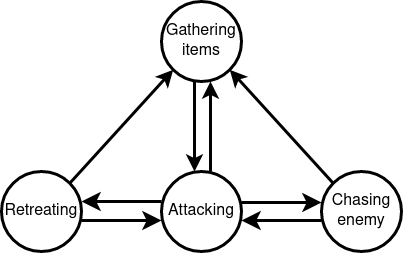
\includegraphics[width=0.4\linewidth]{Images/images/FSM.drawio.png}
\caption{Example of Finite State Machine for a generic bot in an FPS game}
\label{fig:fsm_bot}
\end{center}
\end{figure}
\vspace{1cm}
\begin{figure}
\begin{center}
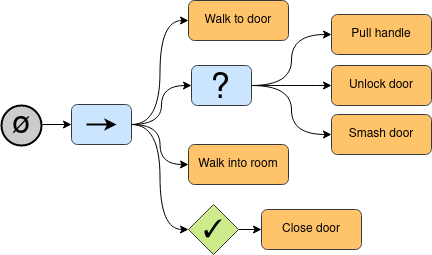
\includegraphics[width=0.5\linewidth]{Images/images/BTTutorial.drawio.png}
\caption{Example of a Behavior tree for the task of entering a closed room.}
\label{fig:tutorial_bt}
\end{center}
\end{figure}
\vspace{1cm}
\begin{figure}
\begin{center}
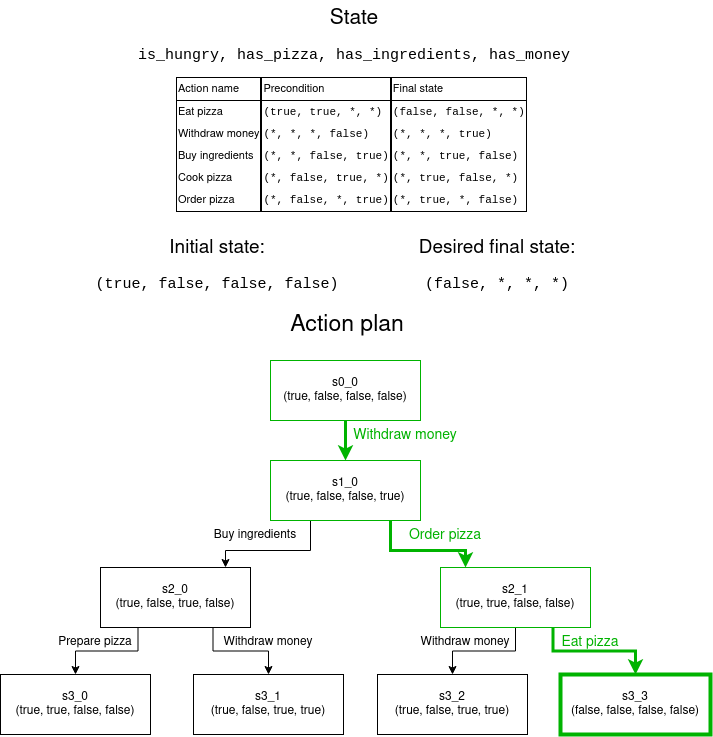
\includegraphics[width=0.8\linewidth]{Images/images/GOAP_NEW.png}
\caption{Example of GOAP to prepare dinner.}
\label{fig:tutorial_goap}
\end{center}
\end{figure}

\subsection{Actuation}
After having chosen the course of action to follow, a bot must take those actions. In order to do so, the bot has to interact with the game engine in order to walk, jump, shoot, reload, and so on.

The actions that a bot can take should subjected to the same limitations a human player has, both accounting for the game rules (e.g. a bot should not move faster than a normal player) and the real world rules (e.g. a bot should not be able to instantly turn around and aim towards an enemy given that this action executed with a mouse would take some time to complete).

\section{Summary}
In this chapter we analysed the high-level architecture of a video game bot, in order to better understand the AI we developed in this research to support our purposes. 
We also briefly discussed some of the nuances of creating a perfect bots versus an enjoyable one in order to understand when either one is more suited.

